\documentclass{midl}
\usepackage{mwe}
\usepackage[english]{babel}
\usepackage{caption}
\usepackage{float}

\title[DLMI]{Lymphocytosis Classification Challenge}

\midlauthor{\Name{Joachim COLLIN} \Email{joachim.collin@eleves.enpc.fr}
\AND
\Name{Bastien LE CHENADEC} \Email{bastien.le-chenadec@eleves.enpc.fr}
}
\begin{document}

\maketitle

\begin{abstract}
\end{abstract}

\section{Introduction}
\label{sec:introduction}

Lymphocytosis is a common hematologic abnormality characterized by an increase in the absolute concentration of lymphocytes to more than 4000 lymphocytes/microL for adult patients \cite{Hamad_2023}. This condition can arise from various sources, including reactions to infections, drugs, or stress, or it may indicate a lymphoproliferative disorder, which is a type of cancer involving abnormal proliferation of lymphocytes. Clinicians typically diagnose lymphocytosis by assessing personal data such as medical history, symptoms, medication lists, and through a blood test to measure lymphocyte levels. However, additional tests may be necessary to confirm the cause of lymphocytosis and determine an appropriate treatment plan. Each condition associated with lymphocytosis presents its own set of symptoms and treatment options. While the diagnosis process is efficient, it suffers from poor reproducibility, and the additional tests required can be costly and time-consuming \cite{Sahasrabudhe_2021}. Being able to distinguish more accurately reactive from malignant lymphocytosis patients is challenging and would lead to a better identification of patients requiring additional testing.

\section{Architecture and methodological components}
\label{sec:methodology}

\subsection{Data preprocessing}

\paragraph*{Annotations}
As a first step in this challenge, we analyze the data distributions to make correct preprocessing and architectural choices. In figure \ref{fig:train_test_histograms}, we observe that the training and test datasets have similar enough distributions of their features (taking into account the small number of samples 163 training samples and 42 testing samples).

\begin{figure}[h]
    \centering
    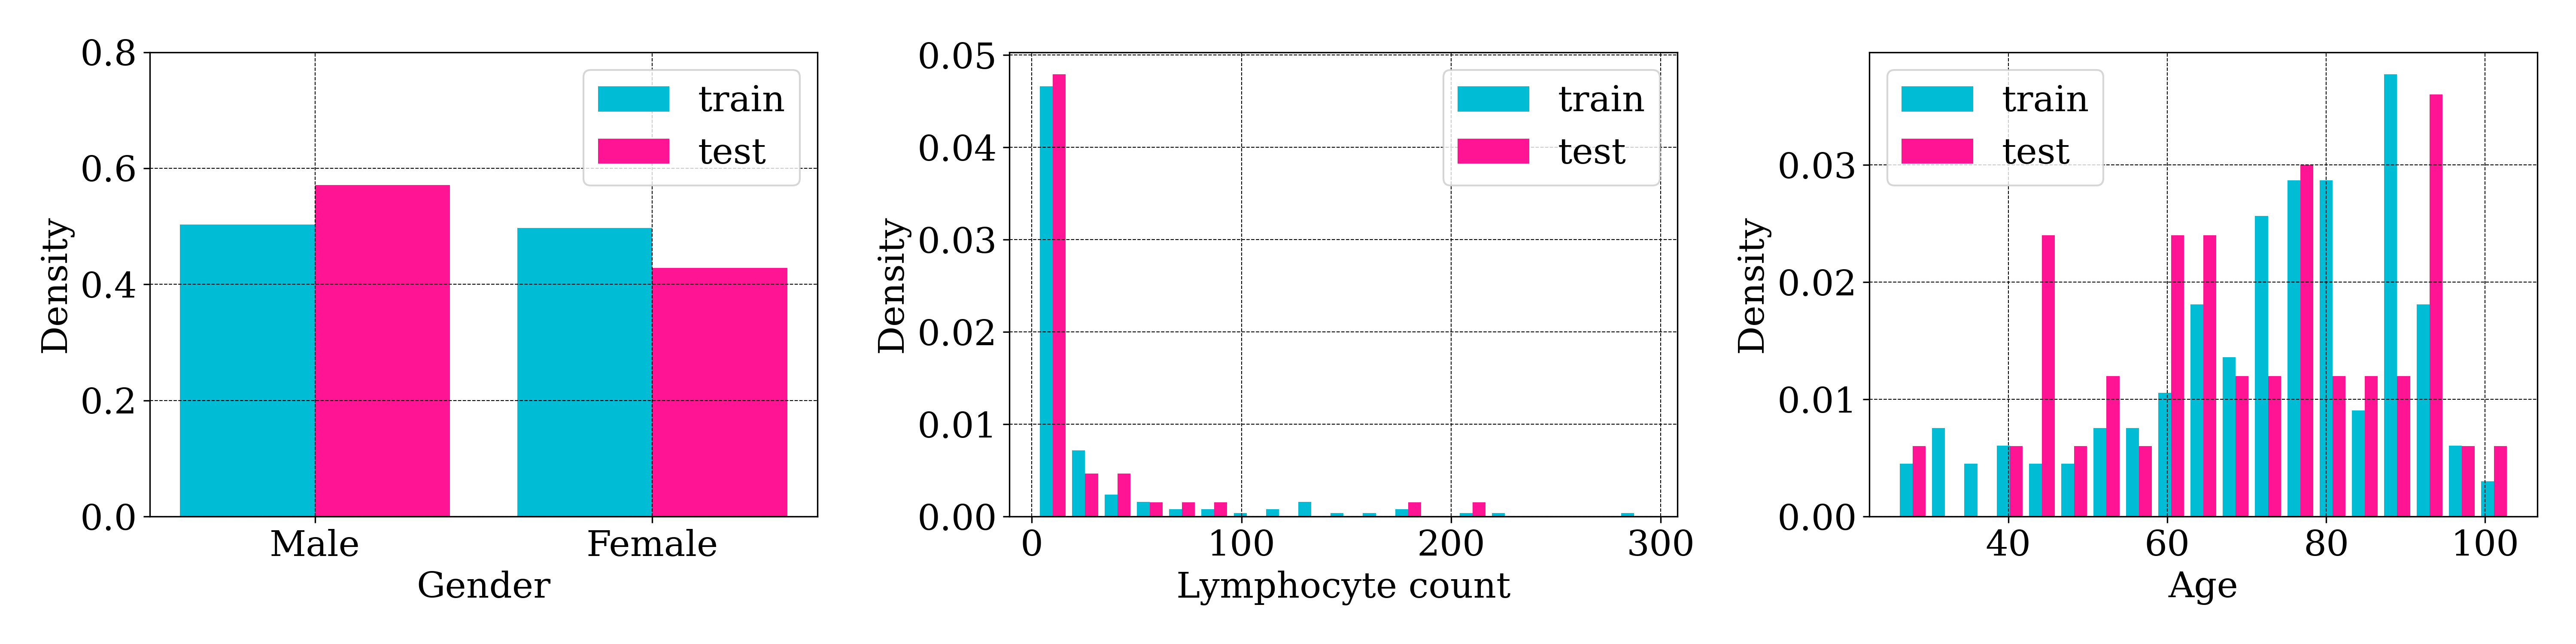
\includegraphics[width=0.9\textwidth]{figures/train_test_histograms.png}
    \caption{Histograms of the training and test datasets.}
    \label{fig:train_test_histograms}
\end{figure}

On figure \ref{fig:positive_negative_histograms}, we observe the distribution of the positive and negative classes in the training dataset. While gender does not seem to be a good predictor of the negative (reactive) or positive (malignant) class, a high lymphocyte count seems to be a good indicator of malignant lymphocytosis. The malignant nature is also more prevalent in older patients.

\begin{figure}[h]
    \centering
    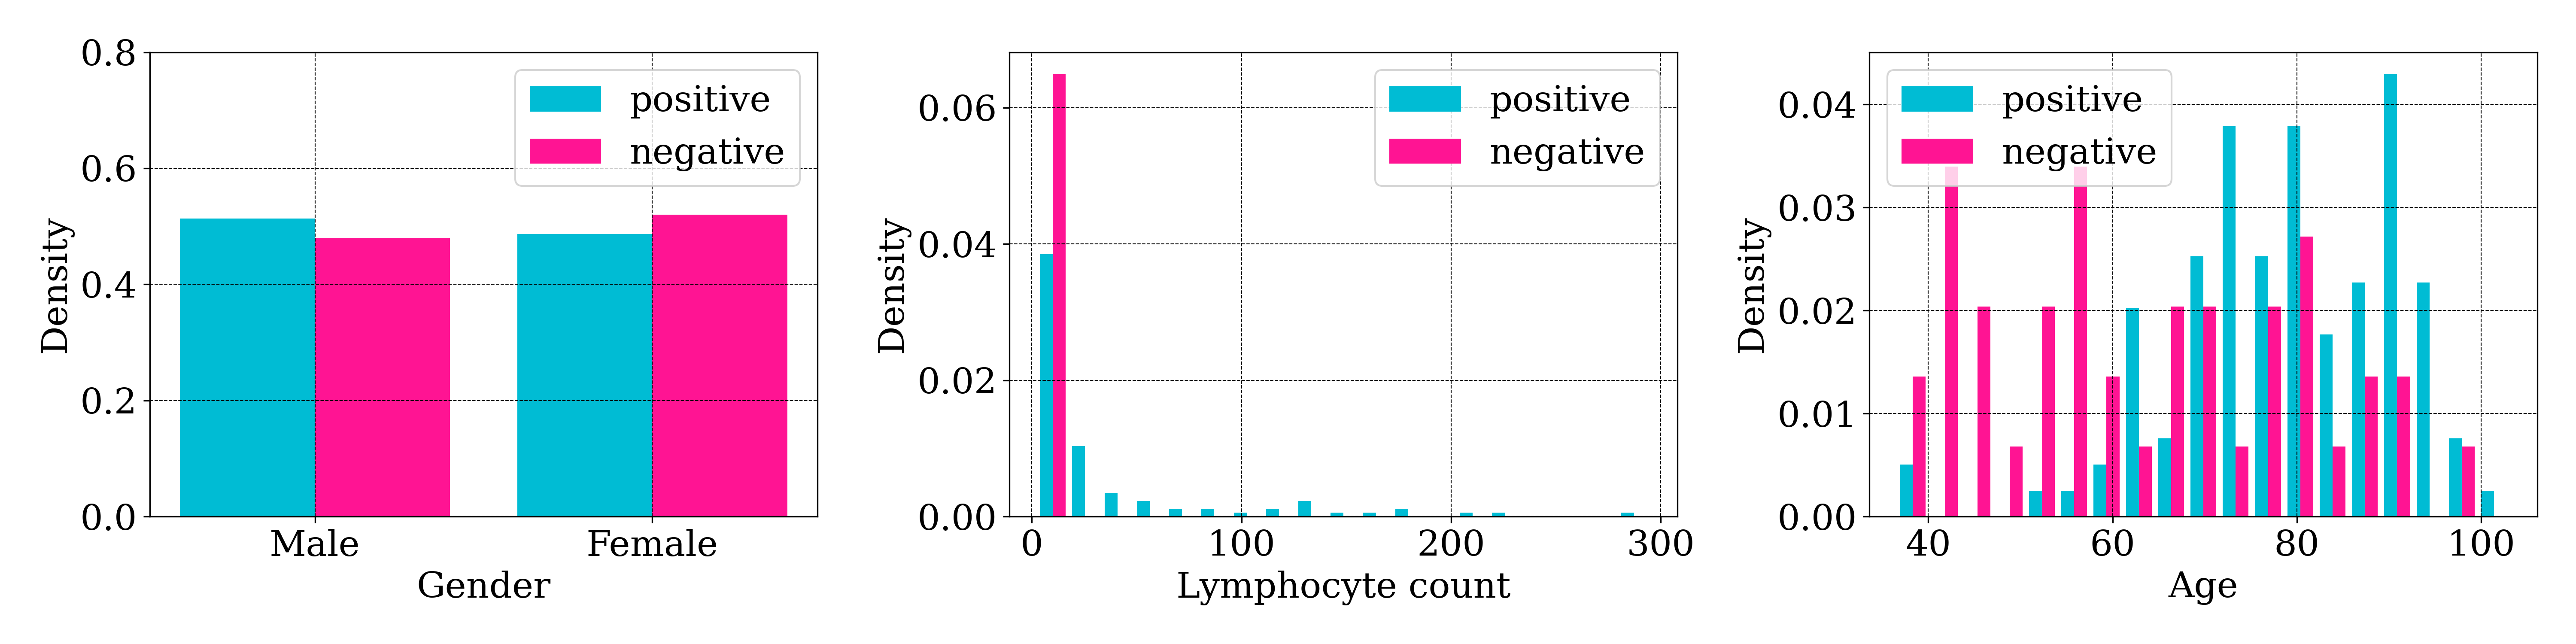
\includegraphics[width=0.9\textwidth]{figures/positive_negative_histograms.png}
    \caption{Histograms of the positive and negative classes in the training dataset.}
    \label{fig:positive_negative_histograms}
\end{figure}

The imbalance between the positive and negative classes ([TODO HOW MUCH]) justifies the use of a \textbf{stratified split} of the training dataset between training and validation sets, i.e. we split the dataset in a way that the proportion of positive and negative classes is the same in the training and validation sets. We also normalize the lymphocyte count and age features to be between 0 and 1.

\paragraph*{Images}
Each patient is associated with a set of images, which are all of size 224x224 pixels. For every deep learning model, we apply the following preprocessing steps, motivated by experimental results:
\begin{enumerate}
    \setlength\itemsep{0em}
    \item \textbf{Normalization}: each image is normalized with standard normalization values (mean = [0.485, 0.456, 0.406], std = [0.229, 0.224, 0.225]).
    \item \textbf{Cropping}: in most images, the relevant information is located in the center of the image (the images are taken by an automatic microscope which centers the cells). We crop the images to a size of 112x112 pixels, which gets rid of 75\% of the pixels while keeping the relevant information.
    \item \textbf{Segmentation} (optional): we applied a segmentation algorithm based on a K-means clustering of the saturation channel of the image. While the segmentation algorithm works well enough, it does not seem to improve the performance of the models, so we do not use it in the final models (See figure \ref{fig:segmentation}).
\end{enumerate}

\subsection{Architectures}

The variable number of images per patient can be seen through two different perspectives: either as a multi-instance learning problem, where the model has to make a prediction based on a set of images, or as a weakly supervised learning problem, where there are missing labels for the images. These perspectives motivate different kind of architectures.

\paragraph*{Baseline}

Our baseline model is a simple convolutional neural network (CNN) with two convolutional layers followed by three fully connected layers. The annotations are concatenated with the output of the last convolutional layer. This model predicts individual labels for each image, and the final prediction is the average of the individual predictions. This model is simple and fast to train, and quickly gives a balanced accuracy of $0.85714$ on the test set.

Building on this baseline, we tried to improve the model by using a more complex architecture (VGG 16, VGG 19) and attention mechanisms, without much success. The limitation of these models is that they do not take into account the set of images as a whole. From a medical perspective, an individual image does not contain enough information to make a diagnosis, and the variety of images per patient is a source of information that should be exploited.

\paragraph*{Unsupervised classification}

Encouraged by the results of the baseline model, we decided to try an unsupervised classification approach. If we can split the images in relevant classes, we can then use a simple machine learning model to predict the class of the patient. We used the state-of-the-art unsupervised classification model SCAN \cite{van-gansbeke-2020}, which is based on a ResNet model. After training the model on our data with 20 class, we computed class confusions based on first and second ranked classes for each image. We then used these confusions to fuse the most similar classes and were left with 15 meaningful classes (figure \ref{fig:unsupervised_classification}). While these classes are not perfect, we hope that they can provide a good enough representation of the data to be used in a simple machine learning model. Using these classes, we compute the following features for each patient:

\begin{itemize}
    \setlength\itemsep{0em}
    \item Gender, lymphocyte count, age (3 features)
    \item Class proportion (15 features)
    \item Entropy of the class distribution (1 feature)
    \item Variety of classes (i.e. number of different image classes for the patient) (1 feature)
    \item Outliers: number of the above features that are greater than 90\% of the same feature in the training samples
\end{itemize}

We run a 5-fold cross-validation with stratified splits and report the balanced accuracy of different machine learning models in figure \ref{fig:unsupervised_classification_models}. There is a lot of variability in the performance of the models, and only one model (GaussianNB) performs better than the baseline on every split. We thus chose to submit a prediction with this model, which has a balanced accuracy of [TODO] on the test set.

\begin{figure}[h]
    \centering
    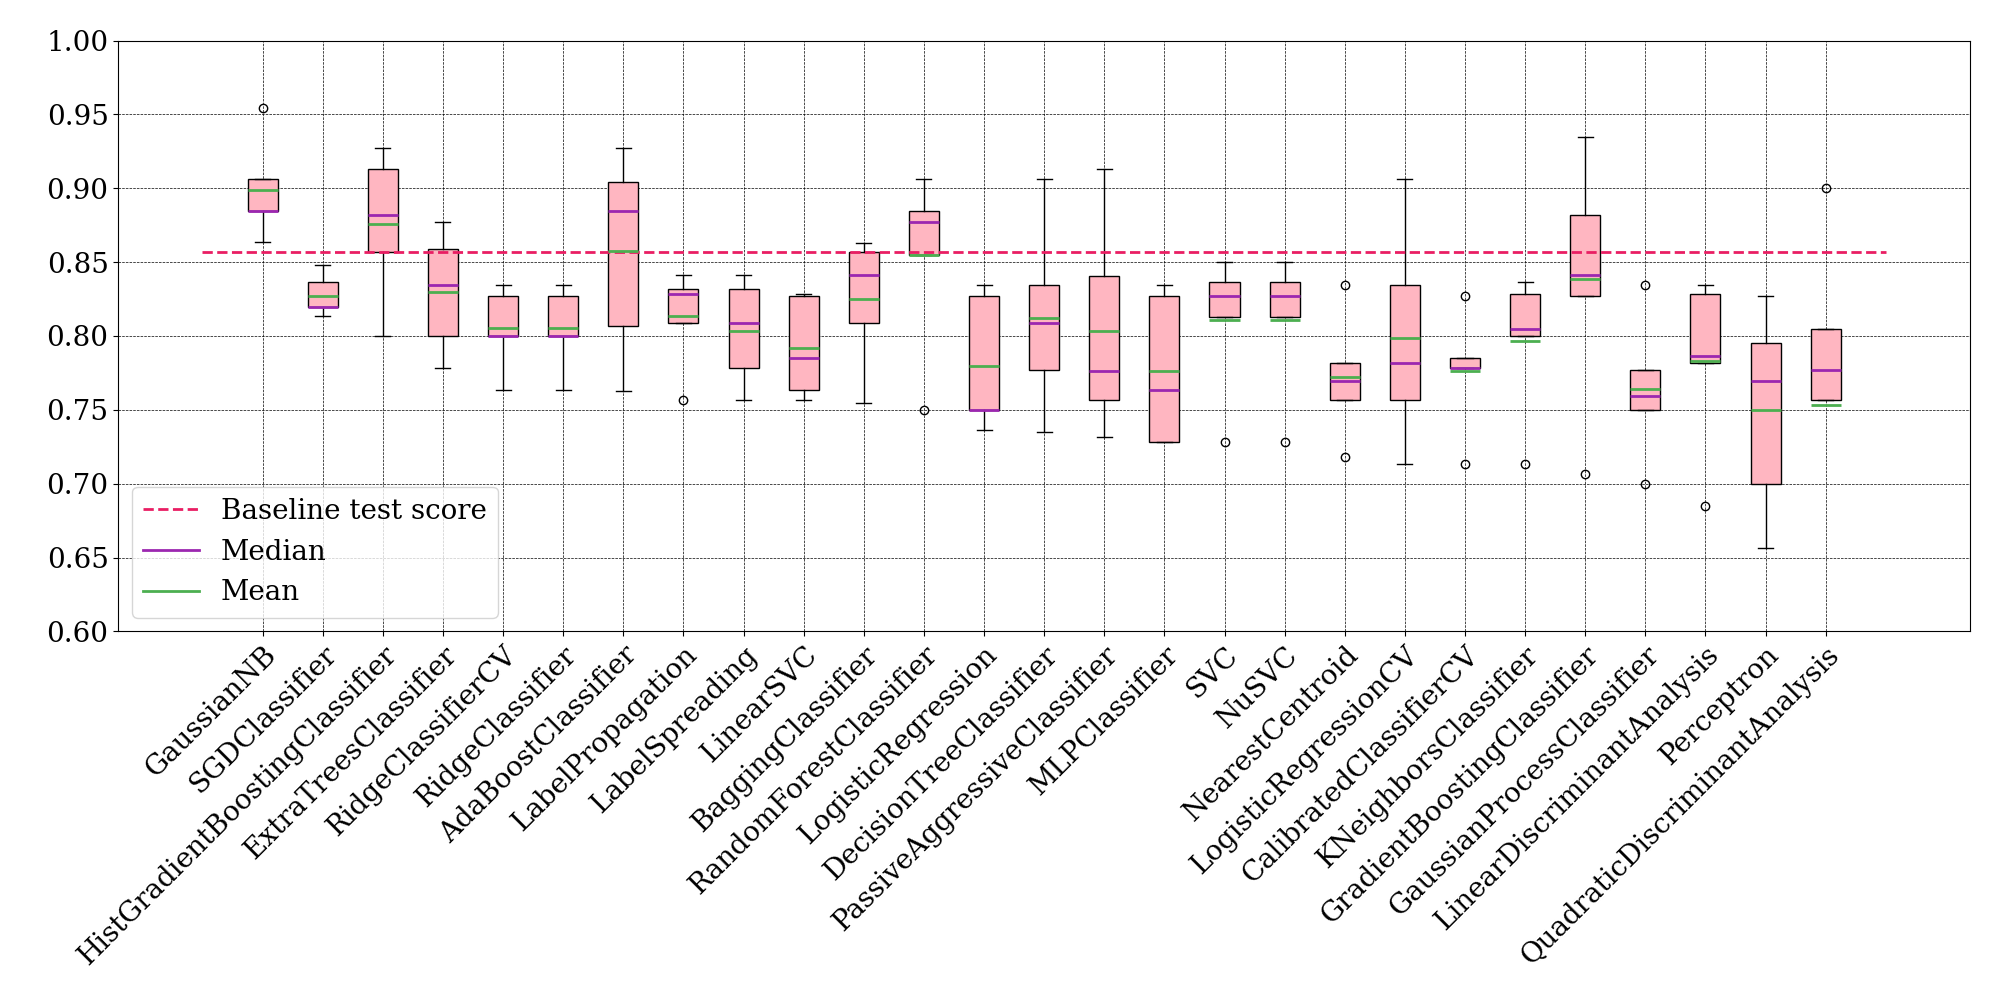
\includegraphics[width=\textwidth]{figures/unsupervised_classification_models.png}
    \caption{Balanced accuracy of different machine learning models on the unsupervised classification features.}
    \label{fig:unsupervised_classification_models}
\end{figure}

\paragraph*{Mixture of experts}
The poor results of the unsupervised classification approach led us back to a deep learning model, but this time we wanted to take into account the set of images as a whole. A natural way to do this is to compute a feature vector for each image, and then to aggregate these feature vectors for instance with mean pooling. We first tried this approach with a model similar to the baseline, but this did not yield good results and the training was very unstable. After some research, we decided to try an architecture inspired by \cite{Sahasrabudhe_2021}. The architecture is detailed in figure \ref{fig:mixture_of_experts}. The model is composed of a feature extractor that operates on images, which are then mean-pooled by patient. The other components are a classifier based on extracted feature maps, a classifier based on patient annotations, and a gating network that decides how to mix the two classifiers.

\begin{figure}[h]
    \centering
    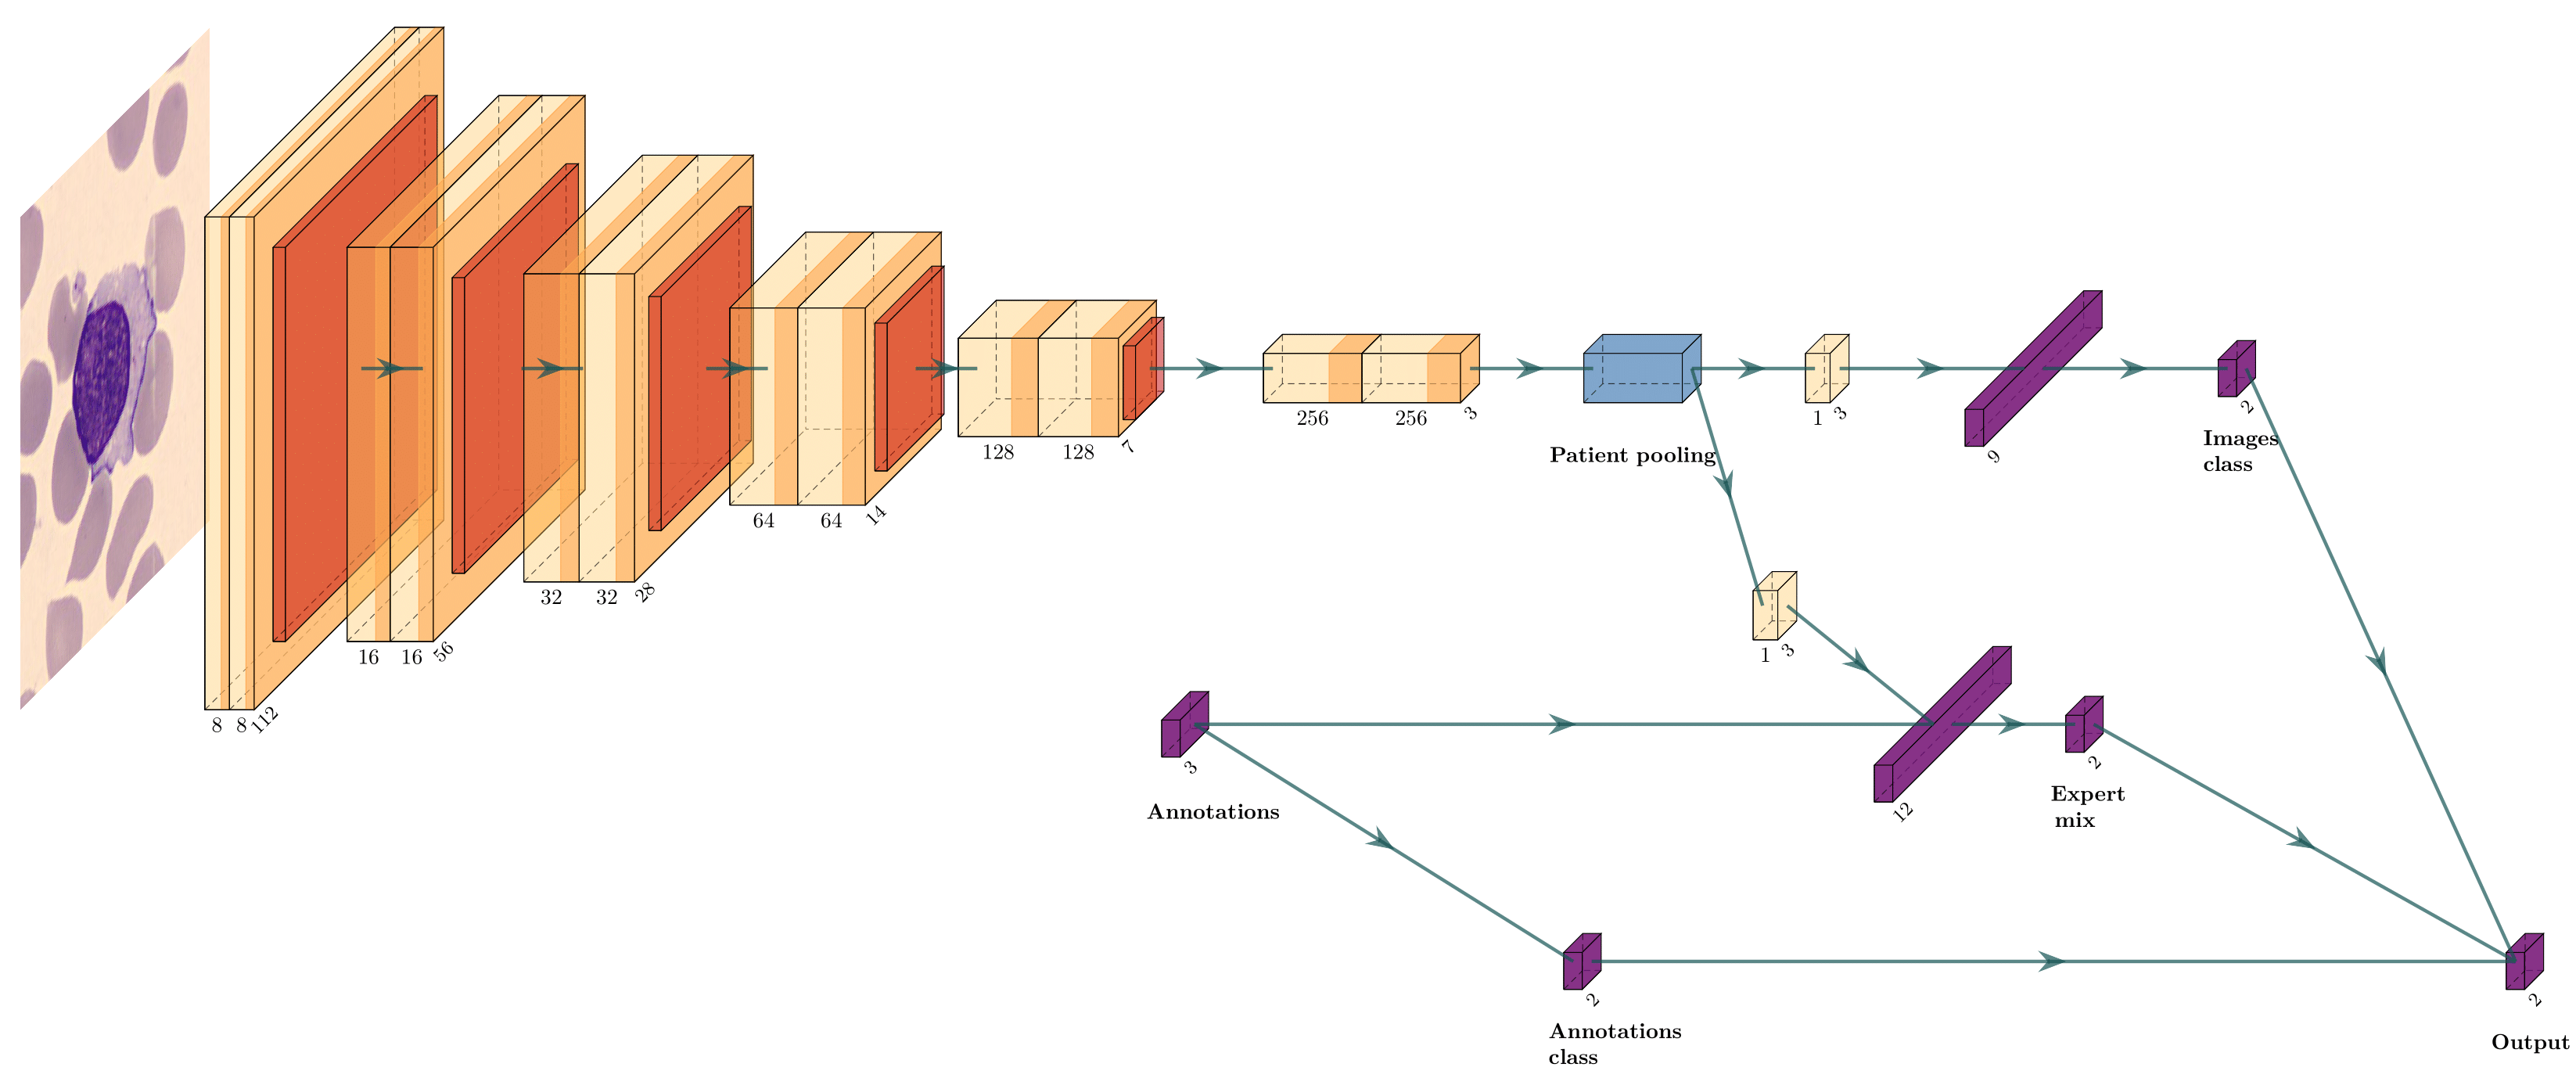
\includegraphics[width=0.9\textwidth]{figures/moe.png}
    \caption{Mixture of experts architecture.}
    \label{fig:mixture_of_experts}
\end{figure}

\section{Model tuning and comparison}
\label{sec:evaluation}

\section{Conclusions}
\label{sec:conclusion}

\newpage
\bibliography{bibliography}

\appendix

\section{Segmentation}

\begin{figure}[H]
    \centering
    {
        \subfigure[Good segmentation][c]{
            \label{fig:good_segmentation}
            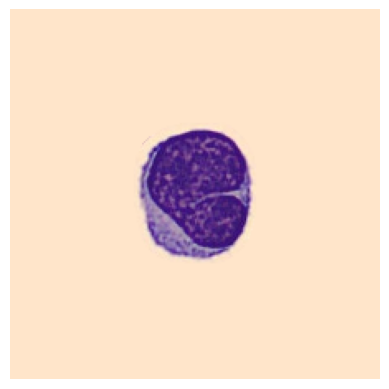
\includegraphics[width=0.25\textwidth]{figures/good_segmentation.png}
        } \qquad
        \subfigure[Bad segmentation][c]{
            \label{fig:bad_segmentation}
            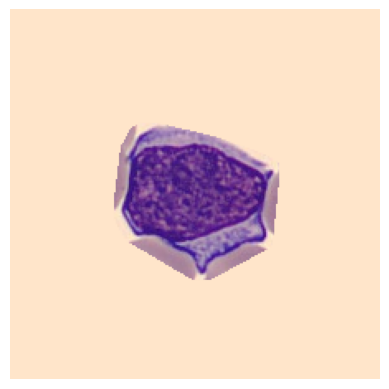
\includegraphics[width=0.25\textwidth]{figures/bad_segmentation.png}
        }
    }
    {\caption{Example of lymphocyte segmentations. On \ref{fig:good_segmentation}, the segmentation is perfect with all the cytoplasm correctly segmented and no left-over pixels. On \ref{fig:bad_segmentation}, the segmentation isn't as great, a lot of blood cell pixels were left to keep all the cytoplasm pixels.\label{fig:segmentation}}}
\end{figure}

\section{Unsupervised classification}

\begin{figure}[H]
    \centering
    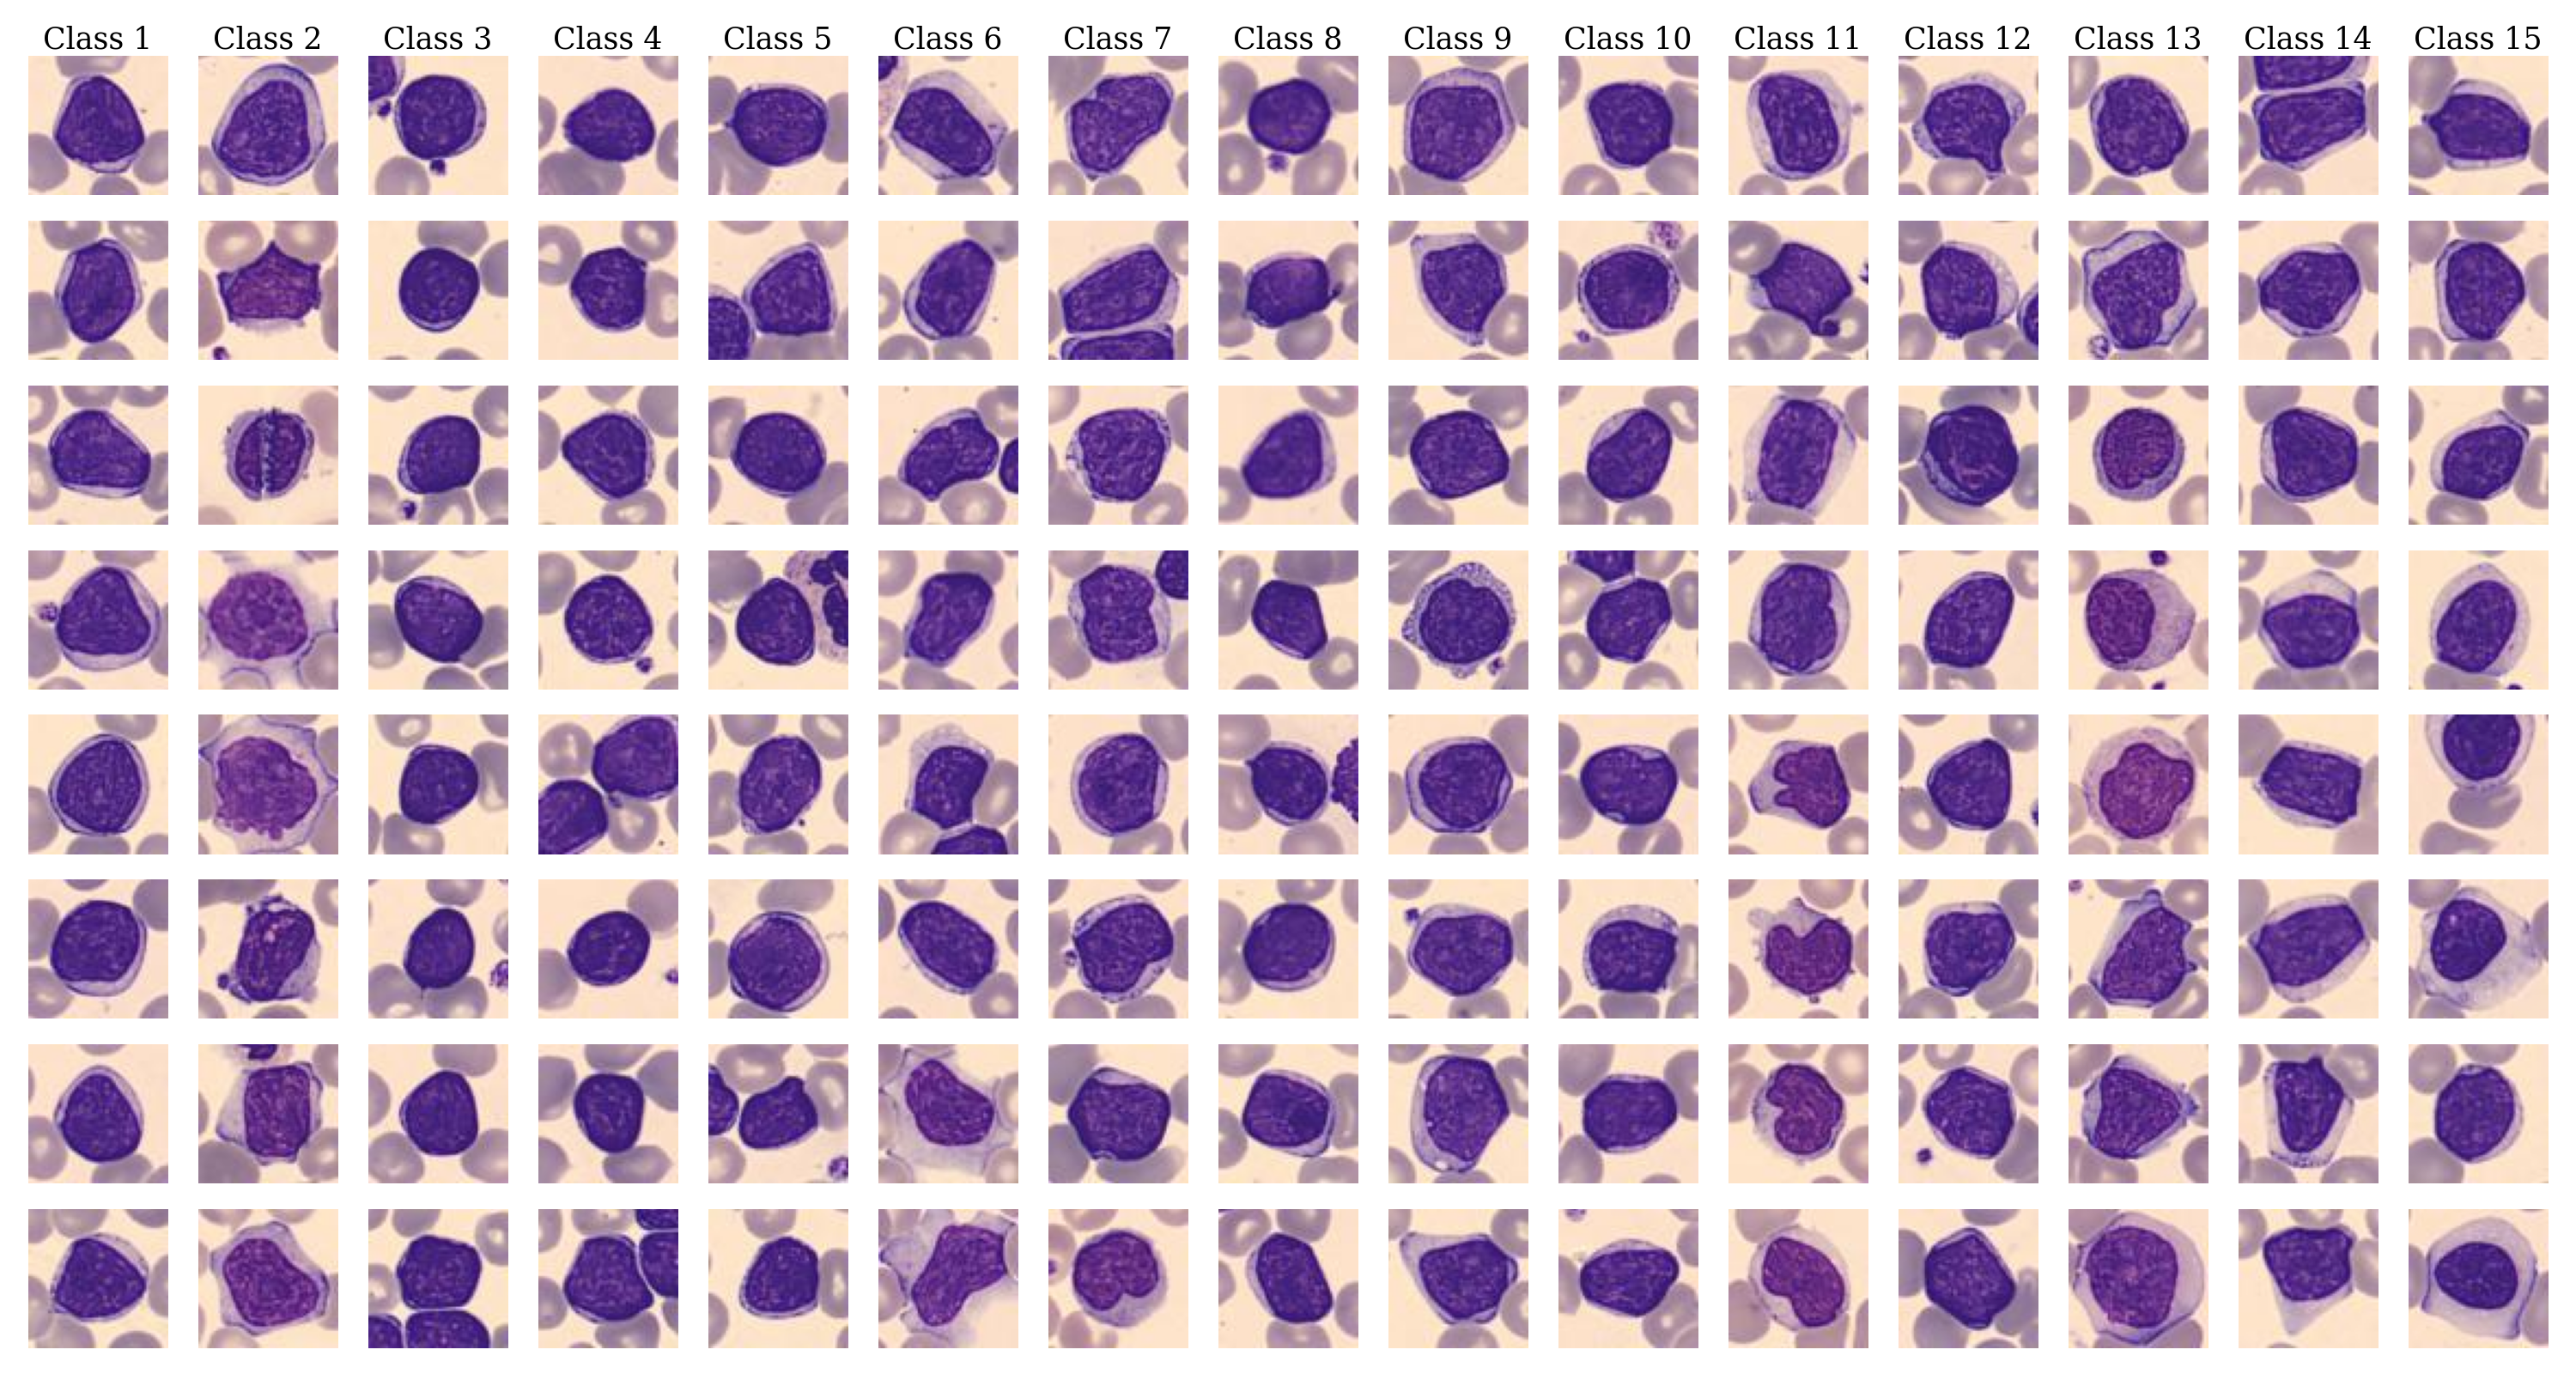
\includegraphics[width=\textwidth]{figures/unsupervised_classification.png}
    \caption{Samples from the 15 classes obtained by unsupervised classification. Each column is a class. We clearly identify some interesting patterns, for instance class 1 is big lymphocytes with medium cytoplasm, class 2 is big lymphocytes with a lot of cytoplasm, class 3 is small lymphocytes with no cytoplasm, etc.}
    \label{fig:unsupervised_classification}
\end{figure}

\end{document}